%%%%%%%%%%%%  Generated using docx2latex.com  %%%%%%%%%%%%%%

%%%%%%%%%%%%  v2.0.0-beta  %%%%%%%%%%%%%%

\documentclass[12pt]{article}
\usepackage{amsmath}
\usepackage{latexsym}
\usepackage{amsfonts}
\usepackage[normalem]{ulem}
\usepackage{soul}
\usepackage{array}
\usepackage{amssymb}
\usepackage{extarrows}
\usepackage{graphicx}
\usepackage[backend=biber,
style=numeric,
sorting=none,
isbn=false,
doi=false,
url=false,
]{biblatex}\addbibresource{bibliography.bib}

\usepackage{subfig}
\usepackage{wrapfig}
\usepackage{wasysym}
\usepackage{enumitem}
\usepackage{adjustbox}
\usepackage{ragged2e}
\usepackage[svgnames,table]{xcolor}
\usepackage{tikz}
\usepackage{longtable}
\usepackage{changepage}
\usepackage{setspace}
\usepackage{hhline}
\usepackage{multicol}
\usepackage{tabto}
\usepackage{float}
\usepackage{multirow}
\usepackage{makecell}
\usepackage{fancyhdr}
\usepackage[toc,page]{appendix}
\usepackage[hidelinks]{hyperref}
\usetikzlibrary{shapes.symbols,shapes.geometric,shadows,arrows.meta}
\tikzset{>={Latex[width=1.5mm,length=2mm]}}
\usepackage{flowchart}\usepackage[paperheight=11.0in,paperwidth=8.5in,left=1.0in,right=1.0in,top=1.0in,bottom=1.0in,headheight=1in]{geometry}
\usepackage[utf8]{inputenc}
\usepackage[T1]{fontenc}
\TabPositions{0.5in,1.0in,1.5in,2.0in,2.5in,3.0in,3.5in,4.0in,4.5in,5.0in,5.5in,6.0in,}

\urlstyle{same}

\renewcommand{\_}{\kern-1.5pt\textunderscore\kern-1.5pt}

 %%%%%%%%%%%%  Set Depths for Sections  %%%%%%%%%%%%%%

% 1) Section
% 1.1) SubSection
% 1.1.1) SubSubSection
% 1.1.1.1) Paragraph
% 1.1.1.1.1) Subparagraph


\setcounter{tocdepth}{5}
\setcounter{secnumdepth}{5}


 %%%%%%%%%%%%  Set Depths for Nested Lists created by \begin{enumerate}  %%%%%%%%%%%%%%


\setlistdepth{9}
\renewlist{enumerate}{enumerate}{9}
		\setlist[enumerate,1]{label=\arabic*)}
		\setlist[enumerate,2]{label=\alph*)}
		\setlist[enumerate,3]{label=(\roman*)}
		\setlist[enumerate,4]{label=(\arabic*)}
		\setlist[enumerate,5]{label=(\Alph*)}
		\setlist[enumerate,6]{label=(\Roman*)}
		\setlist[enumerate,7]{label=\arabic*}
		\setlist[enumerate,8]{label=\alph*}
		\setlist[enumerate,9]{label=\roman*}

\renewlist{itemize}{itemize}{9}
		\setlist[itemize]{label=$\cdot$}
		\setlist[itemize,1]{label=\textbullet}
		\setlist[itemize,2]{label=$\circ$}
		\setlist[itemize,3]{label=$\ast$}
		\setlist[itemize,4]{label=$\dagger$}
		\setlist[itemize,5]{label=$\triangleright$}
		\setlist[itemize,6]{label=$\bigstar$}
		\setlist[itemize,7]{label=$\blacklozenge$}
		\setlist[itemize,8]{label=$\prime$}

\setlength{\topsep}{0pt}\setlength{\parindent}{0pt}

 %%%%%%%%%%%%  This sets linespacing (verticle gap between Lines) Default=1 %%%%%%%%%%%%%%


\renewcommand{\arraystretch}{1.3}


%%%%%%%%%%%%%%%%%%%% Document code starts here %%%%%%%%%%%%%%%%%%%%



\begin{document}
\setlength{\parskip}{8.04pt}
\begin{Center}
\textbf{Barrier Option}
\end{Center}\par

\textbf{Example – Down in Call option(DINC) (Strike price < Barrier Price)}\par

 \( ~P_{DINC}= \left( \frac{H}{S} \right) ^{\frac{2v}{ \sigma ^{2}}} \left( C_{bs} \left[ \frac{H^{2}}{S}, \left( H,K \right) ~ \right] + \left[  \left( H,K \right) ~-K \right] e^{-rt}N \left\{ d_{bs} \left[ \frac{H^{2}}{S}, \left( H,K \right) ~ \right]  \right}  \right) + \left\{ P_{bs} \left( S,K \right) -P_{bs} \left( S,H \right) + \left( H-K \right) e^{-rt}N \left[ -d_{bs} \left( S,H \right)  \right]  \right} B_{H>K}~~ \) \par

Where:\par

H : Barrier Strike Price\par

S : Spot Price\par

\textit{v }:\ r  -  \( \frac{ \sigma ^{2}}{2} \)  \par

r : risk free rate\par

 \(  \sigma  \) : volatility of the underlying asset\par

t : time to maturity\par

 \( C_{bs} \left[ \frac{H^{2}}{S}, \left( H,K \right) ~ \right]  \)  : price of a call option with spot =  \( \frac{H^{2}}{S} \)  and strike =  \(  \left( H,K \right) ~ \)  under Black Scholes model. In which:\par

 \( C_{bs} \left[ \frac{H^{2}}{S}, \left( H,K \right) ~ \right] = \frac{H^{2}}{S}N \left\{ d_{1bs} \left[ \frac{H^{2}}{S}, \left( H,K \right) ~ \right]  \right} -Ke^{-rt}N \left\{ d_{bs} \left[ \frac{H^{2}}{S}, \left( H,K \right) ~ \right]  \right}  \)  \par

 \( d_{bs} \left[ \frac{H^{2}}{S}, \left( H,K \right) ~ \right] =\frac{\ln \ln ~ \left[ \frac{\frac{H^{2}}{S}}{ \left( H,K \right) ~} \right] ~+vt}{ \sigma \sqrt{t}}~~ \) \par

 \( d_{1bs} \left[ \frac{H^{2}}{S}, \left( H,K \right) ~ \right] =d_{bs} \left[ \frac{H^{2}}{S}, \left( H,K \right) ~ \right] + \sigma \sqrt{t}~ \) \par

 \( P_{bs} \left( S,K \right)  \) : price of a put option with spot = S and strike = K under Black Scholes model. In which :\par

 \( P_{bs} \left( S,K \right)  \)  =  \( Ke^{-rt}N \left\{ -d_{bs} \left[ S,K \right]  \right} - SN \left\{ -d_{1bs} \left[ S,K \right]  \right}  \) \par


\vspace{\baselineskip}

\vspace{\baselineskip}

\vspace{\baselineskip}

\vspace{\baselineskip}

\vspace{\baselineskip}

\vspace{\baselineskip}

\vspace{\baselineskip}
Using formula as stated above, let’s price a down-in barrier call option with strike price of $\$$ 90 with spot price $\$$ 100 and down barrier $\$$ 95, risk free interest rate = 6$\%$  and volatility of the underlying asset of 20$\%$  and time to expiration 1 year. Following is the calculation : \par

 \( v=r~ -\frac{ \sigma ^{2}}{2}= 6 \%-\frac{0.2^{2}}{2}=0.04~~  \) \par

 \( \frac{H^{2}}{S}= \frac{95^{2}}{100}=90.25 \)  \par

 \(  \left( H,K \right) ~=  \left( 95,90 \right) ~=95 \) ,\par

 \( d_{bs} \left[ \frac{H^{2}}{S}, \left( H,K \right) ~ \right] =\frac{\ln \ln ~ \left[ \frac{\frac{H^{2}}{S}}{ \left( H,K \right) ~} \right] ~+vt}{ \sigma \sqrt{t}} \)  = -0.0564\par

 \( d_{1bs} \left[ \frac{H^{2}}{S}, \left( H,K \right) ~ \right] =d_{bs} \left[ \frac{H^{2}}{S}, \left( H,K \right) ~ \right] + \sigma \sqrt{t}~ \) = 0.1435\par


\vspace{\baselineskip}
 \( P_{bs} \left( S,K \right)  \)  =  \( Ke^{-rt}N \left\{ -d_{bs} \left[ S,K \right]  \right} - SN \left\{ -d_{1bs} \left[ S,K \right]  \right} = 2.1044 \) \par

 \( P_{bs} \left( S,H \right)  \)  =  \( He^{-rt}N \left\{ -d_{bs} \left[ S,H \right]  \right} - SN \left\{ -d_{1bs} \left[ S,H \right]  \right} = 3.4137 \) \par

 \( C_{bs} \left[ \frac{H^{2}}{S}, \left( H,K \right) ~ \right] = \frac{H^{2}}{S}N \left\{ d_{1bs} \left[ \frac{H^{2}}{S}, \left( H,K \right) ~ \right]  \right} -Ke^{-rt}N \left\{ d_{bs} \left[ \frac{H^{2}}{S}, \left( H,K \right) ~ \right]  \right} =7.5557 \)  \par

Therefore\par

 \( P_{DINC}= \left( \frac{95}{100} \right) ^{\frac{2\ast0.04}{0.20^{2}}} \left( 7.5557+ \left[ 95-90 \right] e^{-0.06\ast1}N \left\{ -0.0564 \right}  \right) + \left\{ 2.1044-3.4137+ \left( 95-90 \right) e^{-0.06\ast1}N \left[ -0.4565 \right]  \right} =9.064667 \) \par


\vspace{\baselineskip}
\textbf{Deriving the Formula}\par

First, We must analyze each compartments in the formula. Mainly, the formula can be separated into two parts which are:\par

\begin{Center}
 \(  \left( \frac{H}{S} \right) ^{\frac{2v}{ \sigma ^{2}}} \left( C_{bs} \left[ \frac{H^{2}}{S}, \left( H,K \right) ~ \right] + \left[  \left( H,K \right) ~-K \right] e^{-rt}N \left\{ d_{bs} \left[ \frac{H^{2}}{S}, \left( H,K \right) ~ \right]  \right}  \right)  \) \ \ \  (1)
\end{Center}\par

\begin{Center}
And
\end{Center}\par

\begin{Center}
 \( + \left\{ P_{bs} \left( S,K \right) -P_{bs} \left( S,H \right) + \left( H-K \right) e^{-rt}N \left[ -d_{bs} \left( S,H \right)  \right]  \right} B_{H>K} \) \ \ \ \ \ \ \ \  (2)
\end{Center}\par


\vspace{\baselineskip}
The separation happens because in pricing down-in call option, The price when option strike price K is lower than the barrier strike price is different than when it is higher. This happens due to the different probability distribution function used when measuring the probability distribution function of the spot price at maturity given the minimum spot price exceeds the barrier strike price during the life of the option and when measuring the probability distribution function of spot price movement at maturity itself. As illustrated below with 95 as spot price, 90 and 87 as the barrier strike price and call option strike price:\par



%%%%%%%%%%%%%%%%%%%% Figure/Image No: 1 starts here %%%%%%%%%%%%%%%%%%%%

\begin{figure}[H]
	\begin{Center}
		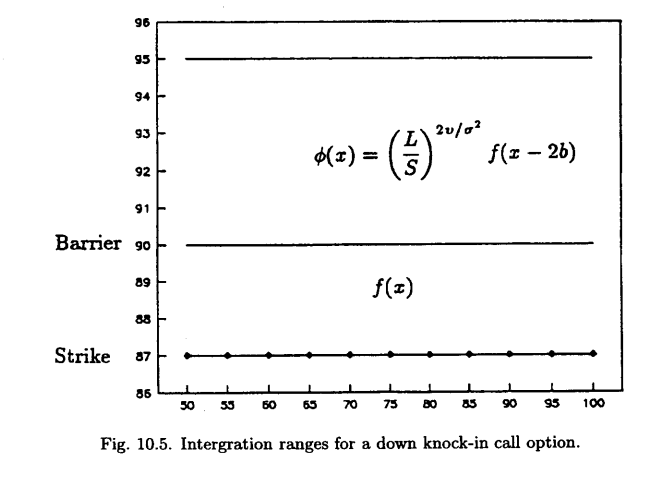
\includegraphics[width=4.94in,height=3.53in]{./media/image1.png}
	\end{Center}
\end{figure}


%%%%%%%%%%%%%%%%%%%% Figure/Image No: 1 Ends here %%%%%%%%%%%%%%%%%%%%

\par

\textbf{Restricted Probability Function  \( f \left( x \right)  \) }\par

Between barrier strike price and call option strike price the probability is measured using the standard normal density function  \( f \left( x \right)  \)  where  \( f \left( x \right) =\frac{1}{ \sigma \sqrt{2 \pi t}}exp⁡ \left[ -\frac{ \left( x-vt \right) ^{2}}{2 \sigma ^{2}t} \right]  \) \ and   \( X_{t}=ln⁡ \left( \frac{S \left( t \right) }{S} \right)  \) . This is the unrestricted distribution used in pricing the normal call option using black scholes method. The formula in (2) tries to calculate the expected payoff of the down in call option from the probability of the price at maturity residing between barrier strike price and call option strike price. \par

\begin{Center}
 \( P_{bs} \left( S,K \right) -P_{bs} \left( S,H \right) + \left( H-K \right) e^{-rt}N \left[ -d_{bs} \left( S,H \right)  \right]  \) 
\end{Center}\par

The pricing formula itself needs to be separated due to in measuring the expected payoff that ranges from (K,$\infty$ ), we have to divide the whole integration range into (K,H) and (H,$\infty$ ) as illustrated in the figures above. Then, for (K,H) we seek the price by separating (K,H) into (-$\infty$ ,H) and (-$\infty$ ,K). By dissecting the formula (2), we know that\par

\begin{Center}
 \(  \left( 2 \right) = Ke^{-rt}N \left\{ -d_{bs} \left[ S,K \right]  \right} - SN \left\{ -d_{1bs} \left[ S,K \right]  \right} -He^{-rt}N \left\{ -d_{bs} \left[ S,H \right]  \right} + SN \left\{ -d_{1bs} \left[ S,H \right]  \right} + \left( H-K \right) e^{-rt}N \left[ -d_{bs} \left( S,H \right)  \right]  \) 
\end{Center}\par

Therefore \par

\begin{Center}
 \(  \left( 2 \right) =SN \left\{ -d_{1bs} \left[ S,H \right]  \right} - SN \left\{ -d_{1bs} \left[ S,K \right]  \right} +Ke^{-rt}N \left\{ -d_{bs} \left[ S,K \right]  \right} -Ke^{-rt}N \left\{ -d_{bs} \left[ S,H \right]  \right}  \) 
\end{Center}\par

Which would be similar to\par

\begin{Center}
 \(  \left( 2 \right) =SN \left\{ d_{1bs} \left[ S,K \right]  \right} -Ke^{-rt}N \left\{ d_{bs} \left[ S,K \right]  \right} - SN \left\{ d_{1bs} \left[ S,H \right]  \right} +Ke^{-rt}N \left\{ d_{bs} \left[ S,H \right]  \right}  \) 
\end{Center}\par

In Which the formula is similar to a call spread of (K, $\infty$ ) and the probability of (H, $\infty$ ) but with K as the strike price.\par

\textbf{Unrestricted Probability Function  \(  \varnothing  \left( x \vert y_{t}>b \right)  \) }\par

For the range (H,$\infty$ ), since the probability we seek is no longer  \( f \left( x \right)  \)  but is\textbf{  \(  \varnothing  \left( x \vert y_{t}>a \right)  \) }. We need to define a new probability density function which is \textbf{  \(  \varnothing  \left( x \vert y_{t}>a \right) =f \left( x \right) - \left( \frac{H}{S} \right) ^{\frac{2v}{ \sigma ^{2}}}f \left( x-2a \right)  \) }. The technique used are named unrestricted probability function because it uses less restriction than the standard normal probability function  \( f \left( x \right) =\frac{1}{ \sigma \sqrt{2 \pi t}}\exp \exp ~ \left[ -\frac{ \left( x-vt \right) ^{2}}{2 \sigma ^{2}t} \right] ~. \)  \par

The idea comes from first deriving the term \par

\begin{Center}
 \( y_{t}=ln⁡ \left( \frac{M_{t}}{S} \right)  \)  and  \( a=ln⁡ \left( \frac{H}{S} \right)  \) 
\end{Center}\par

where  \( M_{t} \)  is the maximum of all underlying asset prices within the life of the option. We then seek for \par

\begin{Center}
 \( P_{t} \left( T_{b}<t \right) =P_{t} \left( M_{t}>H \right) =P_{t} \left( y_{t}>a \right)  \) .\ \  
\end{Center}\par

Harrison(1985) then found that\par

\begin{Center}
 \( F \left( X_{t}<x,~Y_{t}<y \right) =N \left( \frac{x-vt}{ \sigma \sqrt{t}} \right) -e^{\frac{2yv}{ \sigma ^{2}}}N \left( \frac{x-2y- vt}{ \sigma \sqrt{t}} \right)  \) 
\end{Center}\par

That can be differentiated with respect to x into\par

\begin{Center}
 \(  \varnothing  \left( x \vert y_{t}>a \right) =f \left( x \right) - \left( \frac{H}{S} \right) ^{\frac{2v}{ \sigma ^{2}}}f \left( x-2a \right) \text{ for x>a } \) 
\end{Center}\par

And\par

\begin{Center}
 \(  \varnothing  \left( x \vert y_{t}>a \right) =0 for x \leq a \) 
\end{Center}\par


\vspace{\baselineskip}
Furthermore since\par

\begin{Center}
 \(  \varnothing  \left( x \vert y_{t}>a \right) + \varnothing  \left( x \vert y_{t} \leq a \right) =f \left( x \right)  \) 
\end{Center}\par

We can easily build for our down barrier option\par

\begin{Center}
 \(  \varnothing  \left( x \vert y_{t}<a \right) = \left( \frac{H}{S} \right) ^{\frac{2v}{ \sigma ^{2}}}f \left( x-2a \right) \text{ for x>a} \) 
\end{Center}\par

and\par

\begin{Center}
 \(  \varnothing  \left( x \vert y_{t}<a \right) =f \left( x \right)  for x \leq a \) 
\end{Center}\par


\vspace{\baselineskip}
See (Harrison, 1985) for further proof of the new probability function  \(  \varnothing  \left( x \vert y_{t}>b \right) . \) \par


\vspace{\baselineskip}

\vspace{\baselineskip}

\vspace{\baselineskip}
Using the knowledge above, We can better understand the price of (1)\par

\begin{Center}
 \(  \left( \frac{H}{S} \right) ^{\frac{2v}{ \sigma ^{2}}} \left( C_{bs} \left[ \frac{H^{2}}{S}, \left( H,K \right) ~ \right] + \left[  \left( H,K \right) ~-K \right] e^{-rt}N \left\{ d_{bs} \left[ \frac{H^{2}}{S}, \left( H,K \right) ~ \right]  \right}  \right)  \) 
\end{Center}\par

The formula can be analyzed into three different parts. First, the max(H,K) then the  \( ~ \left( \frac{H}{S} \right) ^{\frac{2v}{ \sigma ^{2}}}C_{bs} \left[ \frac{H^{2}}{S}, \left( H,K \right) ~ \right] ~ \) \ and   \(  \left( \frac{H}{S} \right) ^{\frac{2v}{ \sigma ^{2}}} \left[  \left( H,K \right) ~-K \right] e^{-rt}N \left\{ d_{bs} \left[ \frac{H^{2}}{S}, \left( H,K \right) ~ \right]  \right} . \) \par


\vspace{\baselineskip}
The max(H,K) happens simply due to the fact that the probability density function is different when K is above or below H. when K is higher than H, the full price of the down-in call option will simply becomes\par

\begin{Center}
 \( ~ \left( \frac{H}{S} \right) ^{\frac{2v}{ \sigma ^{2}}}C_{bs} \left[ \frac{H^{2}}{S},K \right]  \) 
\end{Center}\par

In which is a standard black scholes pricing formula with additional  \(  \left( \frac{H}{S} \right) ^{\frac{2v}{ \sigma ^{2}}} \)  terms from the restricted probability function and  \( \frac{H^{2}}{S} \) (from the original s) that comes from substituting  \( f \left( x \right)  \)  into  \( f \left( x-2a \right)  \)  or  \( \ln \ln ~ \left( \frac{S}{K} \right) ~into 2a-\ln \ln ~ \left( \frac{K}{S} \right) ~=\ln \ln ~ \left( \frac{H^{2}}{S^{2}} \right) ~-ln⁡ \left( \frac{K}{S} \right)  \) .\par


\vspace{\baselineskip}
If K is lower than H, we would need to also take into account the formula below:\par

\begin{Center}
 \(  \left( \frac{H}{S} \right) ^{\frac{2v}{ \sigma ^{2}}} \left[  \left( H,K \right) ~-K \right] e^{-rt}N \left\{ d_{bs} \left[ \frac{H^{2}}{S}, \left( H,K \right) ~ \right]  \right}  \) 
\end{Center}\par

The formula simply tries to deduct the value of the option using the strike price H-K, but with probability of S higher than H. where the price is not under the unrestricted probability but of the restricted probability distribution function (2).\par


\vspace{\baselineskip}

\vspace{\baselineskip}

\vspace{\baselineskip}

\vspace{\baselineskip}

\vspace{\baselineskip}

\vspace{\baselineskip}

\vspace{\baselineskip}

\vspace{\baselineskip}

\vspace{\baselineskip}

\vspace{\baselineskip}
\textbf{Deriving The Down in Call option(DINC) formula (Strike price < Barrier Price)}\par

Given the down in call option payoff is the positive difference between spot price and strike price at maturity given the spot price has already passed through the barrier price, the payoff should be :\par

\begin{Center}
 \( PDI=max⁡ \{ ⁡ \left[ S_{T}-K,0 \right]  \vert S \left( t \right) >H and S \left( t^{\ast} \right)  \leq H for some t<t^{\ast}<T \}  \) 
\end{Center}\par

Where t is the starting time and T is the time at maturity. Furthermore we can use the Black-Scholes PDE to derive the price. \par

Let  \( \widetilde{W} \)  be a  \( P^{\ast} \) - Brownian motion. As we know, the asset price  \( S_{t} \)  follows the dynamics: \par

\begin{Center}
 \( dS_{t}=S_{t} \left( rdt+ \sigma d\widetilde{W_{t}} \right)  \) 
\end{Center}\par

Which yields\par

\begin{Center}
 \( S_{t}=S_{0}e^{r-\frac{ \sigma ^{2}}{2}t+ \sigma d\widetilde{W_{t}}} \) 
\end{Center}\par

\begin{Center}
 \( P_{DINC}=E^{\ast} \left[ S \left( t \right) \text{>H and }M_{t} \leq \text{H for some t<}t^{\ast}<T \}  \right]  \) 
\end{Center}\par

\begin{Center}
 \( P_{DINC}=e^{-rT}E^{\ast} \left[ ~M_{t} \leq \text{H for some t<}t^{\ast}<T \}  \right]  \) 
\end{Center}\par

\begin{Center}
 \( P_{DINC}=e^{-rT} \int _{0}^{\infty} \int _{-\infty}^{0}P^{\ast} \left[ S_{T}-K \geq x \vert M_{t}-H \leq y \right] dydx \) 
\end{Center}\par

\begin{Center}
 \( P_{DINC}=e^{-rT} \int _{0}^{\infty} \int _{-\infty}^{0}P^{\ast} \left[ S_{T} \geq x+K \vert M_{t} \leq y+H \right] dydx \) 
\end{Center}\par

\begin{Center}
 \( P_{DINC}=e^{-rT} \int _{0}^{\infty} \int _{-\infty}^{0}P^{\ast} \left[ ln\frac{S_{T}}{S_{0}} \geq ln\frac{x+k}{S_{0}} \vert ln\frac{M_{t}}{S_{0}} \leq ln\frac{y+H}{S_{0}} \right] dydx \) 
\end{Center}\par

\begin{Center}
 \( P_{DINC}=e^{-rT} \int _{0}^{\infty} \int _{-\infty}^{0}P^{\ast} \left[ ln\frac{S_{T}}{S_{0}} \geq ln\frac{x+k}{S_{0}} \vert ln\frac{M_{t}}{S_{0}} \leq ln\frac{y+H}{S_{0}} \right] dydx \)  
\end{Center}\par

Let\   \( z=x+k \)  and  \( u=y+H \)  \par

\begin{Center}
 \( P_{DINC}=e^{-rT} \int _{K}^{\infty} \int _{-\infty}^{H}P^{\ast} \left[ ln\frac{S_{T}}{S_{0}} \geq ln\frac{z}{S_{0}} \vert ln\frac{M_{t}}{S_{0}} \leq ln\frac{u}{S_{0}} \right] dydx \) 
\end{Center}\par

Furthermore since\par

\begin{Center}
 \( P_{t} \left( T_{b}<t \right) =P_{t} \left( M_{t}>H \right) =P_{t} \left( y_{t}>a \right)  \) .\ \  
\end{Center}\par

and\par

\begin{Center}
 \( F \left( X_{t}<x,~Y_{t}<y \right) =N \left( \frac{x-vt}{ \sigma \sqrt{t}} \right) -e^{\frac{2yv}{ \sigma ^{2}}}N \left( \frac{x-2y- vt}{ \sigma \sqrt{t}} \right)  \) 
\end{Center}\par

Where\par

\begin{Center}
 \( y_{t}=ln⁡ \left( \frac{M_{t}}{S} \right)  \)  and  \( a=ln⁡ \left( \frac{H}{S} \right)  \) 
\end{Center}\par

Then \par

\begin{Center}
 \( P_{DINC}=e^{-rT} \int _{K}^{\infty} \int _{-\infty}^{H}F \left( X_{t}<x,~Y_{t}<y \right) dydx \) 
\end{Center}\par

\begin{Center}
 \( P_{DINC}=e^{-rT} \int _{ln⁡ \left( \frac{K}{S} \right) }^{\infty} \int _{-\infty}^{\ln \ln ~ \left( \frac{H}{S} \right) ~~}N \left( \frac{x-vt}{ \sigma \sqrt{t}} \right) -e^{\frac{2yv}{ \sigma ^{2}}}N \left( \frac{x-2y- vt}{ \sigma \sqrt{t}} \right) dydx \) 
\end{Center}\par

 \( P_{DINC}= \left( \frac{H}{S} \right) ^{\frac{2v}{ \sigma ^{2}}} \left( C_{bs} \left[ \frac{H^{2}}{S},H \right] + \left[ H-K \right] e^{-rt}N \left\{ d_{bs} \left[ \frac{H^{2}}{S},H \right]  \right}  \right) + \left\{ P_{bs} \left( S,K \right) -P_{bs} \left( S,H \right) + \left( H-K \right) e^{-rt}N \left[ -d_{bs} \left( S,H \right)  \right]  \right} ~~ \) \par

Where  \( d_{bs} \left[ \frac{H^{2}}{S}, \left( H,K \right) ~ \right] =\frac{\ln \ln ~ \left[ \frac{\frac{H^{2}}{S}}{H} \right] ~+vt}{ \sigma \sqrt{t}} \) \par


\vspace{\baselineskip}
\textbf{Example – Down out Call option (DOTC) }\par

Using the knowledge above. Let us price a DOTC with strike prices K = $\$$ 90, spot price = $\$$ 100, and the down barrier = $\$$ 95, with interest rate = 6$\%$  and volatility of 20 $\%$ . We know that the price can be calculated by deriving the formula:\par

 \( P_{DOTC}=C_{bs} \left[ S, \left( H,K \right) ~ \right] - \left( \frac{H}{S} \right) ^{\frac{2v}{ \sigma ^{2}}} \left( C_{bs} \left[ \frac{H^{2}}{S}, \left( H,K \right) ~ \right]  \right) + \left[  \left( H,K \right) ~-K \right] e^{-rt} \left( N \left\{ d_{bs} \left[ S, \left( H,K \right) ~ \right]  \right} - \left( \frac{H}{S} \right) ^{\frac{2v}{ \sigma ^{2}}}N \left\{ d_{bs} \left[ \frac{H^{2}}{S}, \left( H,K \right) ~ \right]  \right}  \right) ~ \) \par


\vspace{\baselineskip}
 \( v=r~ -\frac{ \sigma ^{2}}{2}= 6 \%-\frac{0.2^{2}}{2}=0.04~~  \) \par

 \( \frac{H^{2}}{S}= \frac{95^{2}}{100}=90.25 \)  \par

 \(  \left( H,K \right) ~=  \left( 95,90 \right) ~=95 \) ,\par

 \( d_{bs} \left[ \frac{H^{2}}{S}, \left( H,K \right) ~ \right] =\frac{\ln \ln ~ \left[ \frac{\frac{H^{2}}{S}}{ \left( H,K \right) ~} \right] ~+vt}{ \sigma \sqrt{t}} \)  = -0.0564\par

 \( d_{bs} \left[ S, \left( H,K \right) ~ \right] =\frac{\ln \ln ~ \left[ \frac{S}{ \left( H,K \right) ~} \right] ~+vt}{ \sigma \sqrt{t}} \) \ =  0.4564\par

 \( C_{bs} \left[ S, \left( H,K \right) ~ \right] = SN \left\{ d_{1bs} \left[ S, \left( H,K \right) ~ \right]  \right} -Ke^{-rt}N \left\{ d_{bs} \left[ S, \left( H,K \right) ~ \right]  \right} =12.9871 \) \par

 \( P_{DOTC}=12.9871- \left( \frac{95}{100} \right) ^{\frac{2\ast0.04}{0.2^{2}}} \left( 7.5557 \right) + \left[ 95-92 \right] e^{-0.06\ast1} \left( N \left\{ 0.4564 \right} - \left( \frac{95}{100} \right) ^{\frac{2\ast0.04}{0.2^{2}}}N \left\{ -0.0564 \right}  \right) =7.9855 \) \par

The majority writing in this report are taken from Zhang (1998)\par

\textbf{Reference}\par

Harrison, J.M.,1985, Brownian Motion and Stochastic Flow Systems, Wiley, New York. \par

Zhang, Peter G., 1998, Exotic Options, 2 nd Edition, World Scientific Publishing, Singapore\par


\vspace{\baselineskip}

\printbibliography
\end{document}